%# -*- coding: utf-8-unix -*-
%%==================================================
%% thesis.tex
%%==================================================

% 双面打印
% \documentclass[doctor, fontset=adobe, openright, twoside]{sjtuthesis}
\documentclass[bachelor, fontset=adobe, openany, oneside, submit]{sjtuthesis}
% \documentclass[master, fontset=adobe, review]{sjtuthesis}
% \documentclass[%
%   bachelor|master|doctor,	% 必选项
%   fontset=adobe|windows,  	% 只测试了adobe
%   oneside|twoside,		% 单面打印,双面打印(奇偶页交换页边距,默认)
%   openany|openright, 		% 可以在奇数或者偶数页开新章|只在奇数页开新章(默认)
%   zihao=-4|5,, 		% 正文字号:小四、五号(默认)
%   review,	 		% 盲审论文,隐去作者姓名、学号、导师姓名、致谢、发表论文和参与的项目
%   submit			% 定稿提交的论文,插入签名扫描版的原创性声明、授权声明 
% ]

% 逐个导入参考文献数据库
\addbibresource{bib/thesis.bib}
% \addbibresource{bib/chap2.bib}

\begin{document}

%% 无编号内容:中英文论文封面、授权页
%# -*- coding: utf-8-unix -*-
\title{基于密钥信息的密钥编排方案评估、优化与设计}
\author{陈\quad{}墨}
\advisor{来学嘉教授}
% \coadvisor{某某教授}
\defenddate{2017年6月7日}
\school{上海交通大学}
\institute{电子信息与电气工程学院}
\studentnumber{5130309203}
\major{计算机科学与技术}

\englishtitle{On the Evaluation, Optimization and Design of Key Schedule based on Key Information}
\englishauthor{\textsc{Mo Chen}}
\englishadvisor{Prof. \textsc{Xuejia Lai}}
% \englishcoadvisor{Prof. \textsc{Uom Uom}}
\englishschool{Shanghai Jiao Tong University}
\englishinstitute{\textsc{Depart of Computer Science and Engineering, School of Electronics, Information and Electrical Engineering} \\
  \textsc{Shanghai Jiao Tong University} \\
  \textsc{Shanghai, P.R.China}}
\englishmajor{Computer Science}
\englishdate{Jun. 7th, 2017}


\maketitle

\makeenglishtitle

\makeatletter
\ifsjtu@submit\relax
	\includepdf{pdf/original.pdf}
	\cleardoublepage
	\includepdf{pdf/authorization.pdf}
	\cleardoublepage
\else
\ifsjtu@review\relax
% exclude the original claim and authorization
\else
	\makeDeclareOriginal
	\makeDeclareAuthorization
\fi
\fi
\makeatother


\frontmatter 	% 使用罗马数字对前言编号

%% 摘要
\pagestyle{main}
%# -*- coding: utf-8-unix -*-
%%==================================================
%% abstract.tex for SJTU Master Thesis
%%==================================================

\begin{abstract}

分组密码中常常较为简单的密钥编排方案的低扩散程度常常会导致一些密码攻击。
为了描述与量化这种扩散程度以分析和设计密钥编排方案,黄佳琳等人给出了以实际密钥信息(Actual Key Information)为核心的关于密钥信息的一系列概念。
但是,现有的计算实际密钥信息的算法仍处于贪心(只能给出上界)或是简单枚举的阶段,其正确性和效率性的缺乏限制了其只能用于攻击而不能用于分析、设计编排方案。
在本文中,我们成功地解决了AKI问题这一难题,提出了一个基于图论中著名的最大流问题的一个全新的AKI-最小割算法,同时还进一步给出了一个基于该算法的密钥编排设计方法,旨在设计出一个无密钥信息泄露的密钥编排方案来提供更强的安全性。
作为以上算法的应用,我们成功了优化了对23轮TWINE-80密码的多维零相关线性攻击,并提出了一个新的对12轮RECTANGLE-128的中间相遇攻击。
同时,我们针对以上两个密码及其攻击,分别为这两个密码算法优化、设计了新的密钥编排方案,使其能够抵抗上述攻击,甚至相类似的一系列攻击。

\keywords{\large 分组密码\quad 密钥编排方案 \quad 密钥信息 \quad 实际密钥信息 \quad 最大流问题 \quad 图论 \quad AKI-最小割算法\quad TWINE \quad RECTANGLE \quad 密钥编排方案的优化与设计}
\end{abstract}

\begin{englishabstract}

    The low diffusion of a simplified key schedule in block ciphers is usually responsible for many attacks.
    Huang \emph{et al.} gave conceptions on Key Information, especially the Actual Key Information (AKI), which successfully illustrated and quantified the method to evaluate the diffusion of a key schedule.
    However, the algorithm used to calculate AKI proposed by Huang \emph{et al.} cannot be used to determine the weakness or further make an optimization of a key schedule since it cannot give an accurate value of AKI.
    In this paper, we successfully solve the AKI problem by our AKI - Minimum Cut Algorithm based on the well-known Max-flow problem in Graph Theory,
    and futher give a method to design a key schedule which offers better security with less or without Key Information leakage.
    As applications, we optimize the zero-correlation attack on 23-round TWINE-80 and find a new meet-in-the-middle attack on 12-round RECTANGLE-128,
    and respectively gives a new dependency matrix for TWINE-80 and an optimized key schedule for RECTANGLE-128, which makes both of them stronger against these attacks.

\englishkeywords{\large Block cipher, Key schedule, Key Information, AKI, Max-flow problem, Graph Theory,
    TWINE, RECTANGLE, Design and optimization of key schedules}
\end{englishabstract}



%% 目录、插图目录、表格目录
\tableofcontents
\listoffigures
\addcontentsline{toc}{chapter}{\listfigurename} %将插图目录加入全文目录
\listoftables
\addcontentsline{toc}{chapter}{\listtablename}  %将表格目录加入全文目录
\listofalgorithms
\addcontentsline{toc}{chapter}{算法索引}        %将算法目录加入全文目录

%# -*- coding: utf-8-unix -*-
\begin{symbollist}
\label{chap:symb}

\begin{longtable}{rl}
 $X^j_i$ & $i$轮加密后密文中的第$j$比特 \\
 $K^j_i$ & 第$i$轮轮密钥中的第$j$比特 \\
 $WK^j_i$ & 第$i$轮子密钥中的第$j$比特 \\
 $G(V,E)$ & 由顶点集$V$和边集$E$构成的图$G$ \\
 $K$ & 子密钥集合 \\
 $K_0$ & 密钥信息集合 \\
 $K'_0$ & 实际密钥信息集合 \\
\end{longtable}
\end{symbollist}
 % 主要符号、缩略词对照表

\mainmatter	% 使用阿拉伯数字对正文编号

%% 正文内容
\pagestyle{main}
%\include{tex/intro}
%\include{tex/example}
%\include{tex/faq}
%\include{tex/summary}
%# -*- coding: utf-8-unix -*-
%%==================================================
%% chapter01.tex for SJTU Master Thesis
%%==================================================

%\bibliographystyle{sjtu2}%[此处用于每章都生产参考文献]
\chapter{AKI——实际密钥信息}
\label{chap:AKI}
轮函数的完全扩散性(completeness,即任意一个输出比特都依赖于所有的输入比特)是衡量一个轮函数扩散程度的重要标准。
对于非完全扩散的轮函数,考察其扩散的程度就变得极为重要。
为了精确考察密钥编排方案的弱点导致实际攻击的一般规律,黄佳琳博士在其博士毕业论文\citen{黄佳琳2014分组密码}中提出了实际密钥信息这一概念,从而考察了一个密钥编排方案在给定轮函数时的强弱程度。
\section{AKI的定义}
黄佳琳博士在\citen{huang2014revisiting}中提出了基于密钥依赖路径的实际密钥信息定义,而实际上实际密钥信息可适用于任何子密钥集合。因此,在本节中,我们扩展了黄佳琳博士对AKI的定义:
\begin{defn}[密钥信息集合]
    给定一个子密钥集合$K$,如果通过密钥编排方案,使用另一个子密钥集合$K_0$可以计算出$K$中的所有比特,则称$K_0$是$K$的一个密钥信息集合。
\end{defn}
\begin{defn}[实际密钥信息(AKI)]
    给定一个子密钥集合$K$,其密钥信息集合中最小的集合被成为实际密钥信息集合,实际密钥信息集合的大小即为$K$所包含的实际密钥信息。
\end{defn}
在实际密码攻击方法中,子密钥猜测环节十分常见且重要,例如相关密钥攻击\citen{biham1994new}和中间相遇攻击\citen{diffie1977special}.
在这些攻击中,将子密钥猜测集合替换为其实际密钥信息集合,就可以在不影响猜测的信息的情况下降低需要猜测的比特数量,从而降低攻击的复杂度。
\section{密钥编排方案的密钥信息}
黄佳琳博士在\citen{huang2014revisiting}中提出了使用AKI来分析给定一个轮函数的情况下一个密钥编排方案强弱的方法。
\begin{defn}[计算路径]
    设$O_0$为一个$m$比特的中间状态。根据轮函数我们可以得到一条$O_0$的计算路径:
    $$O_0=f_1(O_1,K_1)=f_1(f_2(O_2,K_2),K_1)=\dots f_1(\dots(f_s(O_s,K_s),K_{s-1}),\dots,K_1),$$
    其中$f_i$依赖于分组密码的结构和第$i$轮的轮函数,而$O_i$, $O_{i-1}$分别为第$i$轮的输入比特集合和输出比特集合。
    $O_0\rightarrow O_1\rightarrow O_2\rightarrow\dots\rightarrow O_s$被成为一条计算路径,其中$O_0$和$O_s$分别为该路径的输出和输入。
\end{defn}
为了构造$O_0$的一条计算路径,我们需要从$O_0$开始往前轮寻找所有计算$O_0$所需要的比特,而这些比特加上$O_0$本身则构成了$O_0$的一条计算路径。
\begin{defn}[密钥依赖路径]
    一条计算路径上所涉及的所有轮密钥比特所构成的集合称为该计算路径的密钥依赖路径。
\end{defn}
密钥依赖路径实际上包含了为了计算$O_0$所需要的所有的轮密钥比特。

一般来说,一个密钥编排方案包含了密钥提取和密钥扩展两个部分。
\begin{defn}[密钥提取]
    密钥提取是密钥编排方案中从第$i$轮的密钥寄存器中的子密钥$WK_i$提取出要使用在轮函数中的轮密钥$RK_i$的过程。
\end{defn}
\begin{defn}[密钥扩展]
    密钥提取是密钥编排方案中从第$i$轮的密钥寄存器中的子密钥$WK_i$生成第$i+1$轮的子密钥$WK_{i+1}$的过程。
\end{defn}
由于对于一个密钥编排方案来说,改变密钥提取方案本质上只是改变了子密钥$WK_i$中比特的顺序,因此为了将目光着重放在密钥扩展上,
在本文中,凡是未提前定义的密钥编排方案,其密钥提取方案默认为简单提取,即$RK_i^j=WK_i^j$。
当密钥提取均为简单提取时,密钥依赖路径的计算就只依赖于轮函数,与密钥编排方案无关,因此给定轮函数的情况下,不同密钥编排方案下同一条密钥依赖路径的实际密钥信息的不同可以用来考察该密钥编排方案在此轮函数情况下的强弱程度。

接下来,我们给出对于一个加密方案,单轮的AKI的定义:
\begin{defn}[单轮实际密钥信息]
    一个加密方案中,第$i$轮的单轮实际密钥信息是该轮中间状态$X_i$中所有单个比特对应的密钥依赖路径的实际密钥信息的最小值。
    \label{def:RoundAKI}
\end{defn}
单轮实际密钥信息描述了该轮所包含的密钥信息的下界。
对于衡量一个密钥编排方案来说,这是一个重要的指标。
我们会在第\ref{chap:App}、\ref{chap:Design}和\ref{chap:Work}章中多次使用这个定义。
为了更方便的计算以上两条路径,我们需要量化轮函数和密钥编排方案中输入比特和输出比特的依赖关系。
\begin{defn}[依赖矩阵]
    一个依赖矩阵$M=M_{i,j}\in\mathbb{F}^{n\times n}_2$包含了单轮输入输出比特之间的依赖关系,其中$M_{i,j}=1$表示第$i$个输出比特依赖于第$j$个输入比特,反之$M_{i,j}=0$表示不依赖。\footnote{值得一提的是,加密算法和解密算法所对应的依赖矩阵不一定互为逆矩阵,需要以实际情况推论。}
\end{defn}
\begin{figure}[htbp]
\centering
    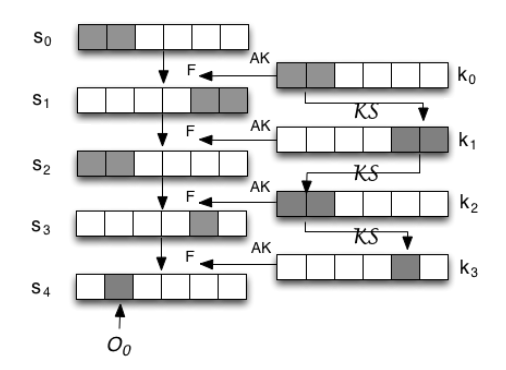
\includegraphics[width=6cm]{ToyCipher}
    \bicaption[fig:toy]{玩具密码}{一个4轮的玩具密码}{ToyCipher}{A 4-round toy cipher}
\end{figure}
\textbf{一个典型的例子\citen{Huang_2014}:}
图\ref{fig:toy}是一个4轮SPN结构的玩具密码,其分组大小和主密钥长度均为6比特,每一个中间状态都直接与相对应的轮密钥进行异或。
其轮函数依赖矩阵为$M_s$,密钥编排方案的依赖矩阵为$M_k$(这里给出了三个不同的编排方案$M_{k1},M_{k2},M_{k3}$)。
$$M_s=\left(
    \begin{array}{cccccc}
        0&0&0&0&0&1\\
        0&0&0&0&1&1\\
        0&0&0&1&0&0\\
        0&0&1&1&0&0\\
        0&1&0&0&0&0\\
        1&1&0&0&0&0
    \end{array}
\right)$$
$$M_k=\left(
    \begin{array}{cccccc}
        0&0&0&0&0&1\\
        0&0&0&0&1&1\\
        0&0&0&1&0&0\\
        0&0&1&1&0&0\\
        0&1&0&0&0&0\\
        1&1&0&0&0&0
    \end{array}
\right)
or\left(
    \begin{array}{cccccc}
        1&0&0&0&0&0\\
        0&1&0&1&0&0\\
        0&0&0&0&1&0\\
        1&0&0&0&0&1\\
        0&0&1&0&0&0\\
        0&0&0&1&0&1
    \end{array}
\right)
or\left(
    \begin{array}{cccccc}
        1&0&1&0&0&0\\
        0&0&0&1&0&0\\
        0&1&0&0&1&0\\
        1&0&0&0&0&0\\
        0&0&1&0&0&1\\
        0&0&0&0&1&0
    \end{array}
\right)$$
令$O_0$只保含了第4轮的第2比特(记为$X_4^1$),我们可以根据轮函数依赖矩阵$M_s$计算出其计算路径:$\{X_0^0,X_0^1\}\rightarrow \{X_1^4,X_1^5\}\rightarrow \{X_2^0,X_2^1\}\rightarrow \{X_3^4\}\rightarrow \{X_4^1\}$。
相对应的,其密钥依赖路径为$\{WK_0^0,WK_0^1\}\rightarrow \{WK_1^4,WK_1^5\}\rightarrow \{WK_2^0,WK_2^1\}\rightarrow \{WK_3^4\}$。
注意到密钥依赖路径中包含了7比特的子密钥,但考虑到主密钥长度只有6比特,因此该密钥依赖路径的所包含的实际密钥信息理论上不可能超过6比特。

在三个密钥编排方案中,密钥编排方案$M_{k1}$由于其与轮函数的依赖关系完全一样,导致密钥依赖路径上各轮比特之间存在与轮函数完全一致的依赖关系,则只用密钥依赖路径在主密钥上的比特就可以推出整条密钥依赖路径。
因此,$\{WK_0^0,WK_0^1\}$就是该密钥依赖路径的一个实际密钥信息集合,AKI仅为2,存在着严重的密钥信息泄露。

而相对的,密钥编排方案$M_{k2}$和$M_{k3}$就表现更好。在编排方案$M_{k2}$下,该密钥依赖路径的AKI为5(其中一个可能的实际密钥信息集合为$\{WK_0^0,WK_0^1,WK_0^2,WK_0^3,WK_0^5\}$),而$M_{k3}$更让AKI达到了理论最大值6。
值得一提的是,$M_{k3}$能够使所有第4轮比特的密钥依赖路径的AKI都达到理论最大值6,即$M_{k3}$使得该玩具密码在经过4轮加密之后不存在任何密钥信息泄露。

因此,AKI不仅在攻击中能够降低某些攻击的复杂度,并且一个密钥编排方案的AKI值也是在某种程度上衡量该方案在其轮函数下的强弱程度的重要参数,而后者中的弱编排方案将会导致该密码函数更容易受到前者的影响,降低攻击该函数的复杂度。
同时,由于给定轮函数后不同的编排方案拥有不同的AKI值,使得AKI成为了设计与优化密钥编排方案的重要指标。

%# -*- coding: utf-8-unix -*-
%%==================================================
%% chapter01.tex for SJTU Master Thesis
%%==================================================

%\bibliographystyle{sjtu2}%[此处用于每章都生产参考文献]
\chapter{AKI算法}
\label{chap:Alg}

为了确定一个子密钥集合$K$的实际密钥信息,我们需要一个算法来计算AKI的值并得到一些可能的实际密钥信息集合。
黄佳琳博士在其博士论文\cite{huang2014revisiting}中提出了一个自动化搜索密钥信息泄露的工具,但该工具设计的算法是一个贪心算法,只能计算出AKI的一个合理上界,无法得到真实的AKI值。
一个AKI的合理上界可以用来进行攻击可能性的分析,但无法用来实际分析一个密钥编排方案的强弱。
Lin等人在\citen{lin2016automatic}中提出了一种对密钥桥技术(Key-Bridging Technique\citen{dunkelman2010improved})的自动化搜索算法,但时间复杂度极高,无法进行大量不同$K$的计算,并且也存在一些反例无法计算(后文中将会提到一个反例)。
因此,现有的AKI算法由于只能给出AKI的一个合理上界,只能用于攻击分析,无法用来分析密钥编排方案的强弱好坏,也不能用来改进密钥编排方案的设计。
本章将会介绍一种全新的基于图论的AKI算法,将会在多项式时间复杂度内计算出真实的AKI值。

\section{单轮加密的AKI}
在介绍完整的AKI算法之前,我们首先从简化版的问题开始考虑——仅有一轮加密时的AKI计算。
我们假设子密钥集合$K$全部集中在第$r$轮上,然后只考虑$r$轮和$r-1$轮两轮之间的依赖关系。
为了解决这个问题,我们将使用图论中二分图的思想来将编排方案、密钥比特、依赖关系等参数量化成图,进而将AKI的计算转化为一个图论的问题。
\begin{defn}[二分图]
    设$G(V,E)$是一个无向图,如果顶点集合$V$可以分割为两个互不相交的子集$A,B$且图中每条边的两个顶点分别属于不同的子集,则称$G$为一个二分图,可记为$G(A,B,E)$。
\end{defn}
\begin{figure}
    \centering
    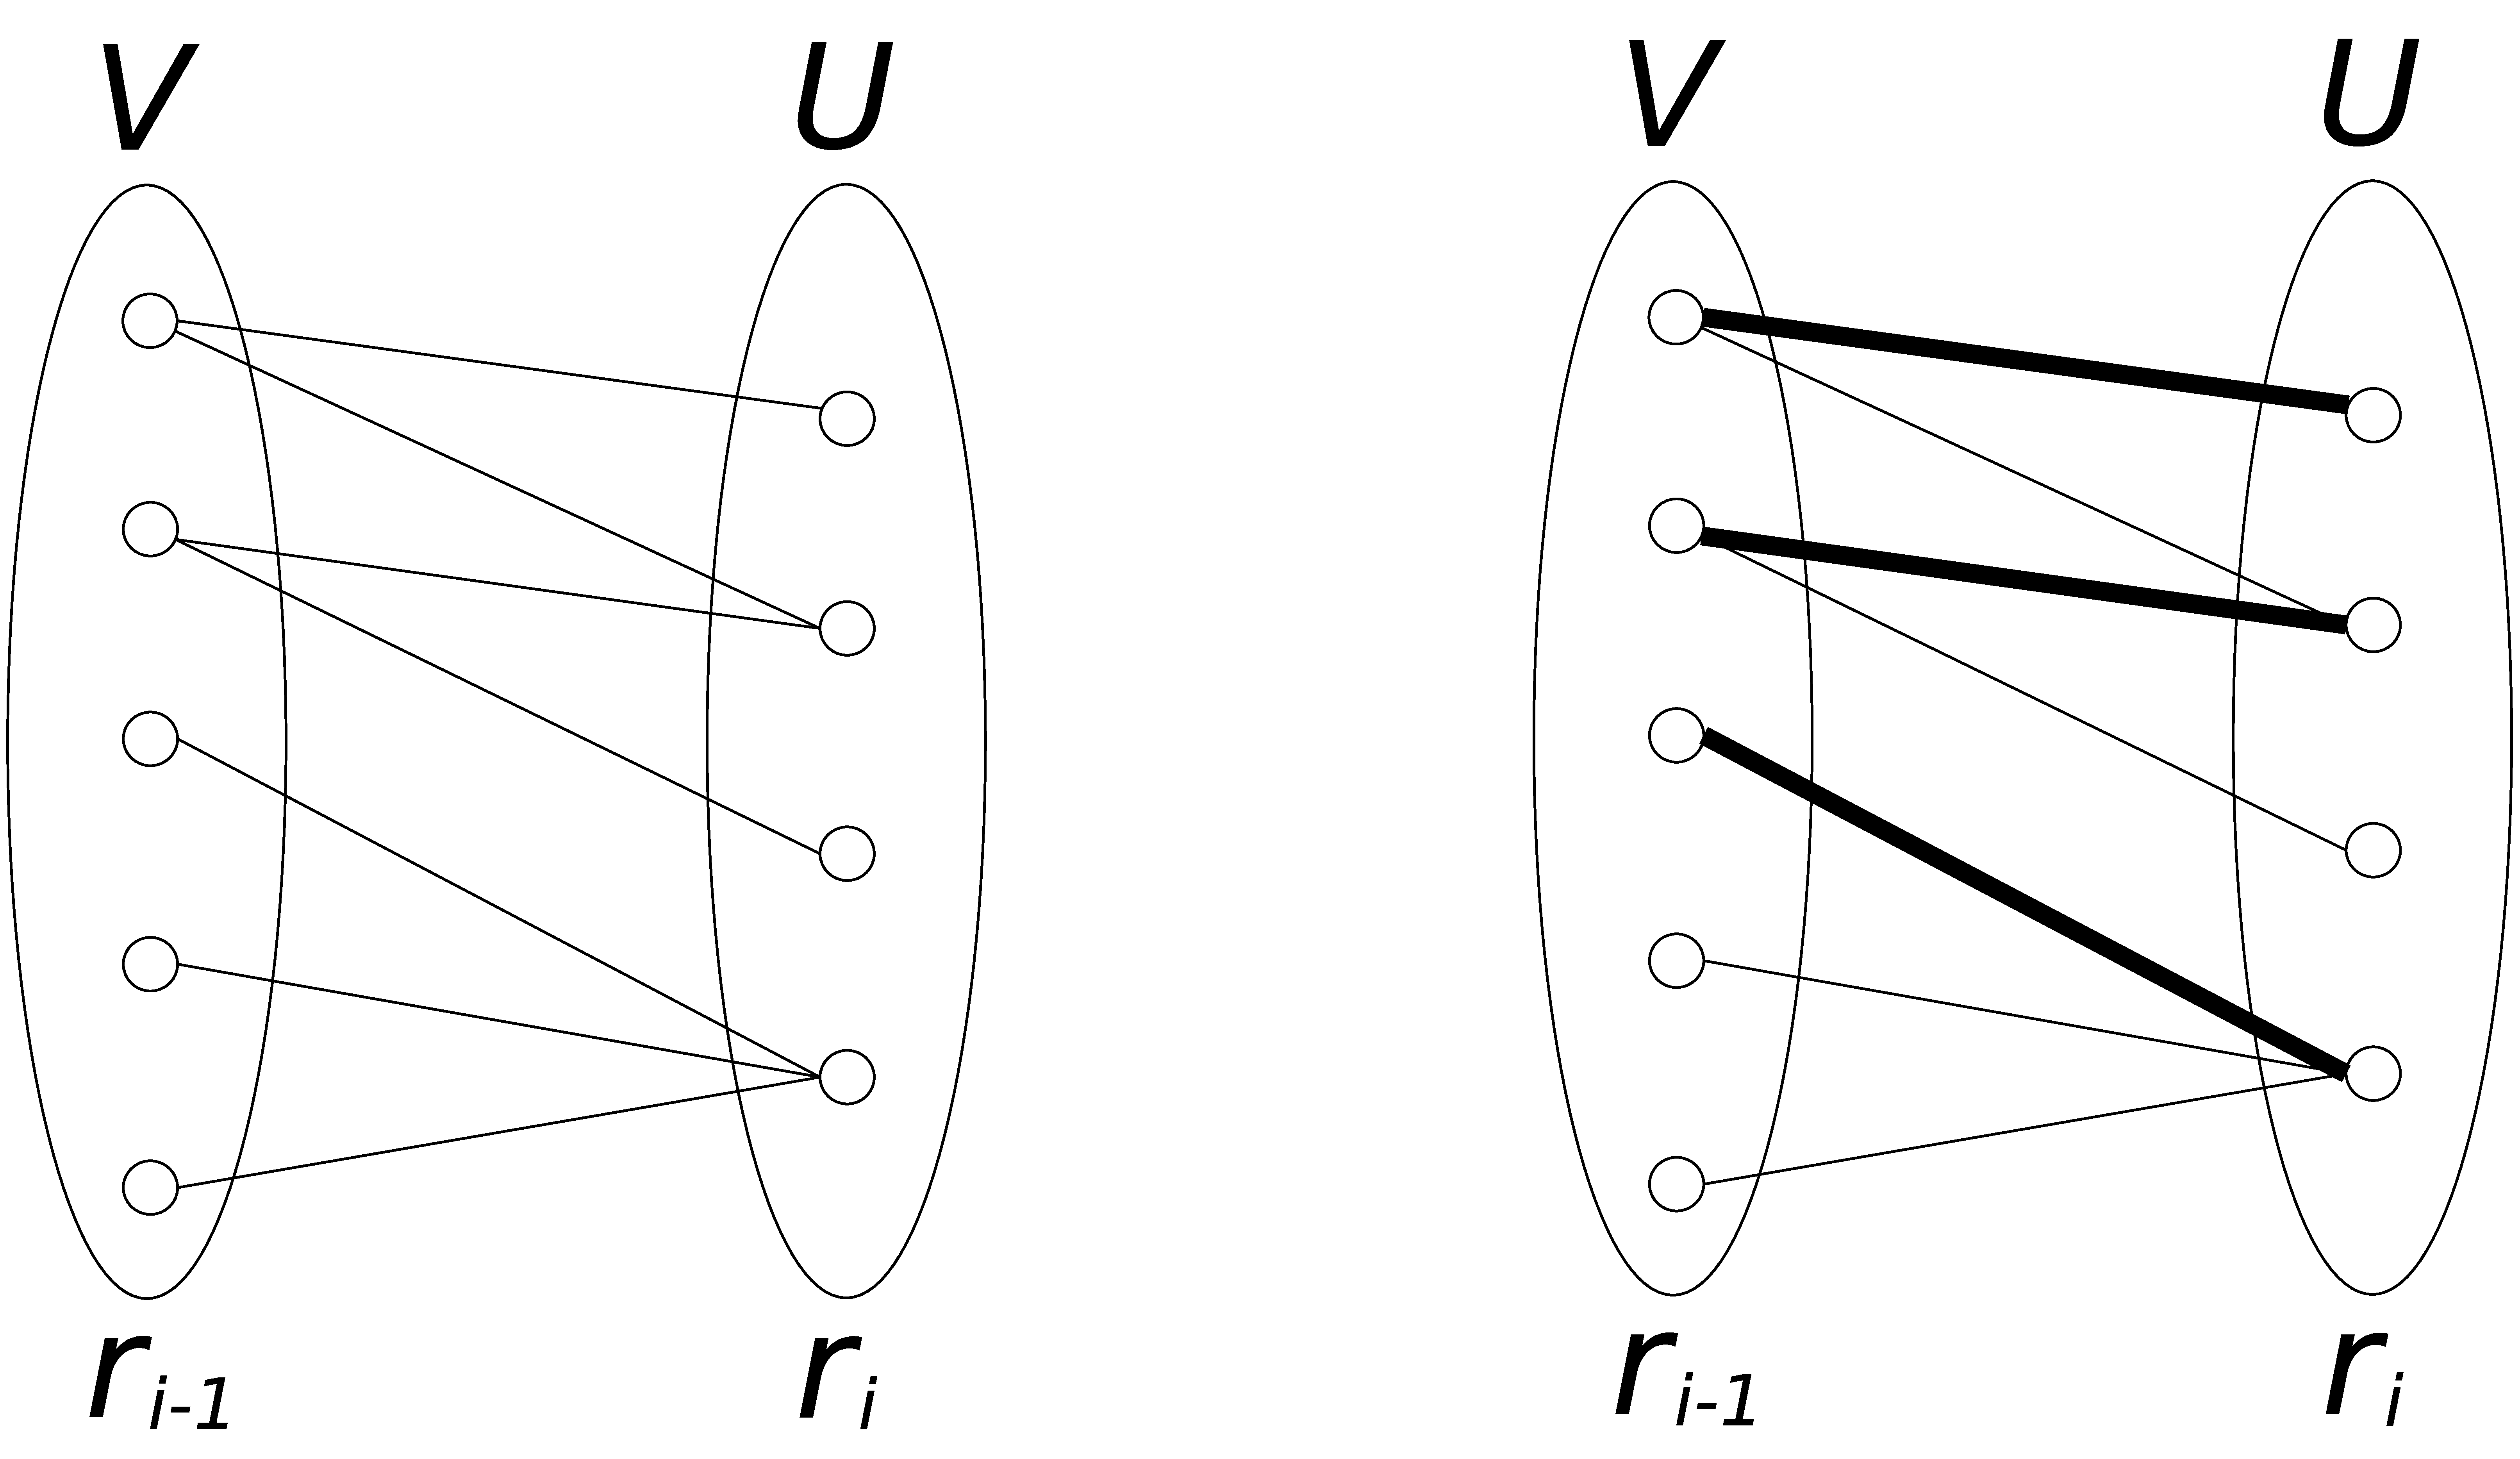
\includegraphics[height=4cm]{bipartite}
    \bicaption[fig:bigraph]{二分图}{一个二分图的例子和它其中一中匹配(被加粗的边)}{Bipartite Graph}{An example of bipartite graph and one of its matching (bold edges)}
\end{figure}
\begin{defn}[图的匹配]
    设$G(V,E)$是一个无向图,如果一个边集$M\subseteq E$中的边两两不相邻(即任意两条边不存在公共的顶点),则成$M$是$G$的一个匹配。
\end{defn}
图\ref{fig:bigraph}中的例子$G(U,V,E)$是一个典型的二分图。我们可以看到所有的边都横跨在两个点集$U,V$之间,而点集的内部不存在任何的边。
在二分图理论中最著名的问题莫过于“二分图最大匹配”问题\citen{west2001introduction},其旨在二分图$G(U,V,E)$中寻找一个最大的匹配$M$。
为了计算最大匹配的值$|M|$,我们需要引入组合数学中著名的霍尔定理\citen{hall1935representatives}的一个拓展:
\begin{thm}[霍尔定理\cite{hall1935representatives}的一个拓展]
    在一个二分图$G(U,V,E)$中,取$U$中的一个子集$X\subseteq U$,记$\Gamma(X)$为$X$的“邻居”,即所有$V$中与$X$中点相邻的点的集合。
    令$\delta(U)=max_{X\subseteq U}\{|X|-|\Gamma(X)|\}$,则有:
    $$MaxMatching(G)=|U|-\delta(U)$$
    \label{thm:hall}
\end{thm}
为了建立轮AKI问题与二分图之间的关系,我们需要这样思考:$r-1$轮和$r$轮的子密钥分别对应子集$V$和$U$中的一个顶点,而这两轮比特之间的一条依赖关系对应横跨$U,V$之间的一条边。
对于给定的子密钥集合$K$(均在$r$轮上),我们把$K$中所有的比特转化成顶点集合$U$,将$K$所依赖的所有$r-1$轮的比特转化为顶点集合$V$,他们之间的依赖关系转化为边集$E$,这样就可以构造出一张二分图$G(U,V,E)$。
这样构造之后,我们重新考虑定理\ref{thm:hall}中的子集$X$(可以视为$K$的一个子比特集合),它的“邻居”$\Gamma(X)$实际上包含了$X$依赖的所有$r-1$轮上的比特,即用$\Gamma(X)$中的所有比特可以推出$X$中的所有比特。
因此,我们可以得出以下引理:
\begin{lem}
    给定一个集中在一轮上的子密钥集合$K$和它的一个子集$X$,令$K'=\Gamma(X)\cup(K\backslash X)$,则$K'$是$K$的一个密钥信息集合。
\end{lem}
\begin{proof}
    由于$\Gamma(X)$可以推出$X$,而$K\backslash X$显然可以推出$K\backslash X$本身,则$K'$可以推出$K$,因此$K'$是$K$的一个密钥信息集合。
\end{proof}
为了找出$K$的实际密钥信息集合,我们需要找到一个最小的密钥信息集合。由于
$$|K'|=|K|-|X|+|\Gamma(X)|=|K|-(|X|-|\Gamma(X)|)$$
又由前文构造出的图$G(U,V,E)$,我们可以得到实际密钥信息集合$K'_{min}$必然满足:
\[
\begin{split}
    |K'_{min}|&=min\{|K|-|X|+|\Gamma(X)|\}\\
              &=|U|-max_{X\subseteq U}\{|X|-|\Gamma(X)|\}\\
              &=|U|-\delta(U)=MaxMatching(G) \qquad\ref{thm:hall}
\end{split}
\]
因此,一个子密钥集合$K$的实际密钥信息的值等于由$U=K$构造出的二分图$G(U,V,E)$的最大匹配的值,且实际密钥信息集合为$K'_{min}=\Gamma(X_{max})\cup(K\backslash X_{max})$,其中$X_{max}$是使$|X|-|\Gamma(X)|$最大的$X$。

\section{AKI-最小割算法}
aaaaa


\appendix	% 使用英文字母对附录编号,重新定义附录中的公式、图图表编号样式
\renewcommand\theequation{\Alph{chapter}--\arabic{equation}}	
\renewcommand\thefigure{\Alph{chapter}--\arabic{figure}}
\renewcommand\thetable{\Alph{chapter}--\arabic{table}}
\renewcommand\thealgorithm{\Alph{chapter}--\arabic{algorithm}}

%% 附录内容,本科学位论文可以用翻译的文献替代。
\include{tex/app_setup}
\include{tex/app_eq}
\include{tex/app_cjk}
\include{tex/app_log}

\backmatter	% 文后无编号部分 

%% 参考资料
\printbibliography[heading=bibintoc]

%% 致谢、发表论文、申请专利、参与项目、简历
%% 用于盲审的论文需隐去致谢、发表论文、申请专利、参与的项目
\makeatletter

%%
% "研究生学位论文送盲审印刷格式的统一要求"
% http://www.gs.sjtu.edu.cn/inform/3/2015/20151120_123928_738.htm

% 盲审删去删去致谢页
\ifsjtu@review\relax\else
  %# -*- coding: utf-8-unix -*-
\begin{thanks}

本人的学位论文是在我的导师来学嘉教授的指导下完成的。
感谢来教授用丰富的专业知识指导我完成对密钥编排方案的深度探究,从开题到构思、撰写和定稿,来教授都给了我莫大的帮助。
来教授渊博的学识与对学术兢兢业业的态度,激励着我向信息安全领域进一步求学的信念。

感谢闫海伦学姐的指导,在与闫海伦学姐讨论中,我学到的不仅是丰富的专业知识,还学到了作为一个研究者应有的态度和努力。

最后感谢我的家人在此期间给予我的包容、关爱和鼓励,以及所有陪我一路走来的同学和朋友,
正是由于他们的支持和照顾,我才能安心学习,并顺利完成我的学业。

\end{thanks}
 	  %% 致谢
\fi

\ifsjtu@bachelor
  % 学士学位论文要求在最后有一个英文大摘要,单独编页码
  \pagestyle{biglast}
  %# -*- coding: utf-8-unix -*-
\begin{bigabstract}
The low diffusion of a simplified key schedule in block ciphers is usually responsible for many attacks.
    Huang \emph{et al.} gave conceptions on Key Information, especially the Actual Key Information (AKI), which successfully illustrated and quantified the method to evaluate the diffusion of a key schedule.
    However, the algorithm used to calculate AKI proposed by Huang \emph{et al.} cannot be used to determine the weakness or further make an optimization of a key schedule since it cannot give an accurate value of AKI.
    In this paper, we successfully solve the AKI problem by our AKI - Minimum Cut Algorithm based on the well-known Max-flow problem in Graph Theory,
    and further give a method to design a key schedule which offers better security with less or without Key Information leakage.
    As applications, we optimize the zero-correlation attack on 23-round TWINE-80 and find a new meet-in-the-middle attack on 12-round RECTANGLE-128,
    and respectively give a new dependency matrix for TWINE-80 and an optimized key schedule for RECTANGLE-128, which makes both of them stronger against these attacks.

A key schedule is an algorithm that expands a relatively short master key to a large expanded key as round keys used in encryption and decryption algorithms.
When it comes to block ciphers, the key schedules are often simplified due to implementation considerations and cause weakness that can be exploited in many attacks, especially for lightweight block ciphers since their schedule are designed based on not only the security but also the effciency of software and hardware.
Key schedules like that of PRESENT\citen{Bogdanov}, RECTANGLE\citen{zhang2015rectangle}, TWINE\citen{Suzaki_2013} and LBlock\citen{Wu_2011} are round-by-round iterations with low diffusion;
Key schedules like that of SIMON and SPECK\citen{beaulieusimon} have simple permutations or linear operations with low diffusion.
Some ciphers like LED\citen{Guo2011} do not even have a key schedule, and just use master keys directly in each round.
Those key schedules are simple and efficient but responsible for many attacks, especially related-key attack\citen{biham1994new,Biryukov2009,Ko2004} and meet-in-the-middle attack\citen{diffie1977special,Biryukov2015,Bogdanov2011}.

In order to illustrate and quantify the diffusion and the detailed weakness which should be responsible for the genetic attacks, Huang \emph{et al.} gave conceptions on Key Information in \citen{huang2014revisiting}, including Computation Path, Key Dependency Path and Actual Key Information, which vividly described the diffusion of a key schedule. 
Taking use of the Key Information leakage of key schedules, Huang \emph{et al.} derived meet-in-the-middle attacks on 40-round SHACAL-2\citen{Handschuh2002} and 25-round XTEA\citen{Needham1997} in \citen{huang2014revisiting} and further proposed an algorithm in \citen{Huang_2014} which could give a reasonable upper bound of the AKI of a key schedule.
However, to design a key schedule which offers more security in Key Information, an accurate value of AKI is required and a method or principle for such a design is essential.

\noindent
\textbf{Our Contribution}. In this paper, we demonstrate a polynomial algorithm solving the AKI problem based on Graph Theory, building a "bridge" between key schedules and flow networks.
We describe the method solving AKI problem from the highly simplied version problem of 1-round AKI, and prove the equivalence between 1-round schedule and bipartite graph.
Further, we introduce the Max-flow Min-cut Theorem and give our AKI - Mimimum Cut Algorithm.
A theoretical proof of the correctness of our algorithm is also included.
By calculating the accurate AKI, we optimize the zero-correlation attack on 23-round TWINE-80 and derive a new meet-in-the-middle attack on 12-round RECTANGLE-128.

Meanwhile, taking use of the "bridge" between key schedules and flow networks we build, we give a greedy algorithm which can generate a new schedule (presented in dependency matrix) from a given subkey set without Key Information leakage.
Based on this algorithm, we respectively give a new matrix for TWINE-80 against the zero-correlation attack and a new key schedule for RECTANGLE-128 which makes any meet-in-the-middle attack on more than 8 rounds impossible.

The source code of the algorithms mentioned above is available \href{https://github.com/KirisameNanami/AKI-Algorithms}{here}.

In order to determine the existance of Key Information leakage, there are several algorithms to compute AKI.
Huang has given an automatic detection tool which includes the calculation of AKI in \citen{Huang_2014}, but the algorithm was a greedy algorithm, which means that it could only give a possible upper bound of AKI.
Also, the Automatic Search of Key-Bridging Technique\citen{dunkelman2010improved} proposed by Lin \emph{et al.} in \citen{lin2016automatic} could also find an upper bound of AKI (since a key bridge is exactly 1-bit leakage of Key Information).
However, neither of the two algorithm could compute the accurate value of AKI (a counterexample will be provided in following sections), which made them a tool for generating an attack such as meet-in-the-middle attack \citen{diffie1977special}, but not for evaluating the safety of a key schedule.
Also, the low efficiency of both of the algorithms (usually several minutes for a single subkey set) limit the application to a whole key schedule, since we have to examine the KDPs from all the internal bits.
In this paper, we will demonstrate our AKI - Minimum Cut Algorithm based on Graph Theory which can get the accurate value of AKI.
This AKI algorithm is based on graph theory, aims at transform the key schedule (represented by the dependency matrix $M$) and a subkey bits set $K$ to a directed flow graph $G_f(E,V,c)$.
Algorithm .~\ref{alg:const} is used to construct such graph.
Briefly speaking, besides the two completely new vertex $s$ and $t$, we construct two vertex $u_{in},u_{out}$ for each bit which is or is depended by the bits in $K$ according to the key schedule $M$, and connect them from $u_{in}$ to $u_{out}$ with a capacity of 1.
All the other edge has its capacity of infinity, and there're three kinds of those edges:
\begin{enumerate}
    \item Edge from $s$ to $u_{in}$ where $u$ is in first round,
    \item Edge from $u_{out}$ to $t$ where $u\in K$,
    \item Edge from $u^{b}_{out}$ to $u^{b'}_{in}$ where $b$ and $b'$ are in two consecutive rounds and $b'$ depends on $b$ according to the key schedule.
\end{enumerate}

For a subkey set $K$ and a dependency matrix $M$ of a $n$-bit key schedule, let $R$ be the maximum round on which bits in $K$ are.
Then the graph $G_f$ constructed by Algorithm.~\ref{alg:const} will have at most $2nR$ vertices (each bit has two vertices and there are at most $R\cdot n$ bits) and $n+|K|+nR+n^2R$ edges (consider the situation that $M$ is a full matrix).
Currently there are many algorithms to solve Max-flow problem. The Push Relabel Algorithm (with highest label node selection rule) has its performance of $\mathcal{O}(V^2\sqrt{E})$ in time complexity, where $V$ and $E$ stands for the number of vertices and edges, respectively.
Hence, the time complexity for our AKI - Minimum Cut algorithm will be $\mathcal{O}((2nR)^2\sqrt{n+|K|+nR+n^2R})=\mathcal{O}(n^3R^{2.5})$, which is polynomial.
It guarantees that for most encryption methods, our algorithm can terminate in seconds.

Since the AKI-set plays the same role with the subkey set $K$ in Key Information, once there exists a leakage of Key Information, the complexity of an attack based on a guessing set $K$ (usually with a distinguisher whose input/output is the set which $K$ is generated from) will be easily reduced by replacing $K$ by its AKI-set $K'_0$.
In this paper, we will introduce two applications based on Key Information leakage.

After we quantify the key schedule with a flow network constructed by Algorithm.~\ref{alg:const}, we can further consider how to design a key schedule with the best performance in terms of AKI.
Theoretically, for a key schedule with a $n$-bit master key and a subkey set $K$, if $|K|\geq n$, there must exist a key schedule with its dependency matrix $M$ which makes the AKI of $K$ be $n$.
This conclusion is trivial since a full matrix (all the cells are 1) $M_{full}$ obviously meet the requirments.
However, such a full matrix $M_{full}$ cannot be used in practical as a dependency matrix of a key schedule.
Hence, we need to find a matrix with the number of '1's as small as possible.

In this paper, we give a new algorithm to give the accurate value of AKI defined by Huang \emph{et al.}, which can be used not only to evaluate and determine the diffusion of a key schedule, but also to optimize the subkey set used in attacks like related-key attack.
We also gives a new method to optimize and re-design a key schedule without Key Information leakage.
To demonstrate the usefulness of those methods, we optimize the zero-correlation attack on 23-round TWINE-80 and generate a new meet-in-the-middle attack on 12-round RECTANGLE-128,
and respectively give new key schedules for both of them which make them secure enough against their attacks.

Although, to the best of our knowledge, we only provide the method of finding a possible, relatively small dependency matrix on a certain subkey set,
we still believe that the "bridge" we built between key schedules and flow networks will work further in summarizing a scientific, theoretical and complete serial of principles on designing the key schedule for a round function.

\end{bigabstract}

\else
  % 盲审论文中,发表学术论文及参与科研情况等仅以第几作者注明即可,不要出现作者或他人姓名
  \ifsjtu@review\relax
    \include{tex/pubreview}
    \include{tex/projectsreview}  
  \else
    \include{tex/pub}	      %% 发表论文
    \include{tex/projects}  %% 参与的项目
  \fi
\fi

% \include{tex/patents}	  %% 申请专利
% \include{tex/resume}	  %% 个人简历

\makeatother

\end{document}
